\documentclass[11pt,a4paper]{article}

\usepackage{amsmath,amssymb,amsthm}
\usepackage{hyperref}
\usepackage{booktabs}
\usepackage{graphicx}
\usepackage{microtype}

\newtheorem{theorem}{Theorem}[section]
\newtheorem{proposition}[theorem]{Proposition}
\newtheorem{corollary}[theorem]{Corollary}
\newtheorem{lemma}[theorem]{Lemma}
\theoremstyle{definition}
\newtheorem{definition}[theorem]{Definition}
\newtheorem{remark}[theorem]{Remark}

\newcommand{\bstar}{\beta^*}
\newcommand{\dhat}{\hat{\delta}}
\newcommand{\Heis}{\mathrm{Heis}_3}
\newcommand{\ZqZ}{\mathbb{Z}/q\mathbb{Z}}
\newcommand{\Fq}{(\mathbb{Z}/q\mathbb{Z})^*}

\title{Fibre Admissibility and Resolution of the Capacity Exponent Discrepancy\\
\large O16 --- Spectral Admissibility Subprogram}

\author{J.~Beau\\
\small Independent Researcher}

\date{2026}

\begin{document}

\maketitle

\begin{abstract}
The O-series has established that the Weil-block capacity exponent
$\dhat_{\mathrm{exact}} \approx 3.72 \pm 0.06$ falls systematically
below the phenomenological target range $\delta \in [7.4, 10.6]$,
and that this discrepancy is structural: no reweighting of block data
can raise the exponent (O15, Corollary~4.8).
The present paper resolves the discrepancy by identifying a
misidentification of the physically relevant observable.
The non-injectivity of the projection~$\Pi$, established from the
Born--Infeld constraint, implies that admissibility is a property
of complete fibres of~$\Pi$, not of individual preimage configurations.
In the Weil realisation of $\Heis(\ZqZ)$, these fibres are organised
as conjugate pairs $\{c, q-c\}$ under the exact identity
$\rho_{q-c} = \overline{\rho_c}$.
The pair-level observable $\sigma_{\mathrm{pair}}(n) = \sigma_c(n)\,\sigma_{q-c}(n)$
follows a clean power law with exponent $\delta_{\mathrm{pair}} = 2\,\delta_c
\approx 7.44 \pm 0.12$, confirmed numerically with $R^2 > 0.9999$ and a
factor-of-six reduction in slope variance.
This result does not modify the underlying model; it identifies the
correct unit of observation.
\end{abstract}

\tableofcontents

\section{Context and statement of the problem}
\label{sec:context}

The O-series investigates the cascade exponent~$\bstar$ and the
capacity exponent~$\delta$ governing projective dynamics on discrete
Heisenberg group Cayley graphs over $\ZqZ$ for prime~$q$.
Papers O12--O15~\cite{Beau2026a16,Beau2026a17,Beau2026a18}
established the following chain of results.
(O12~\cite{Beau2026a16}, O13~\cite{Beau2026a17}, and
O14/O15~\cite{Beau2026a18} are referenced individually where precision
is required.)

\begin{enumerate}
\item The Weil-block redundancy $\sigma_c(n)$ measured at BFS shell~$n$
for a block of character~$c$ decays as a power law
$\sigma_c(n) \sim C_c\, n^{-\delta_c}$ in the pre-saturation regime.

\item The arithmetic mean $\bar\sigma(n) = m_{\mathrm{block}}^{-1}
\sum_c \sigma_c(n)$ is the observable currently extracted by the pipeline.
The exponent $\dhat$ fitted from $\bar\sigma(n)$ satisfies
$\dhat_{\mathrm{exact}} \approx 3.72 \pm 0.06$ universally across
$q \in \{29, 61, 101, 151, 211\}$.

\item This value is structurally below the phenomenological target
$\delta \in [7.4, 10.6]$.
O15 Corollary~4.8 (aggregation no-go) establishes that no reweighting
of block data raises $\dhat$ above $\dhat_{\mathrm{exact}}$,
eliminating arithmetic corrections as a resolution.
\end{enumerate}

The present paper identifies the source of the remaining discrepancy
and resolves it through a redefinition of the observable, dictated
by the non-injectivity structure of~$\Pi$ already present in the
Born--Infeld framework~\cite{Beau2026a2}.
Papers O12--O15 correctly compute the admissible capacity at the level
of individual spectral blocks.
The result below shows that the physically relevant observable lives
at the level of \emph{conjugate pairs}, without modifying the
underlying construction.
A key diagnostic is that a genuine asymptotic power law emerges only
at the pair level: at the level of individual blocks, the log-log
scaling exhibits significant drift (local-slope standard deviation
$\approx 0.98$), while the pair-level observable achieves a
six-fold reduction in slope variance and a power law with
$R^2 > 0.9999$.

\section{Non-injectivity and fibre structure}
\label{sec:fibre_structure}

\subsection{The parity involution from Born--Infeld non-injectivity}

The projection $\Pi : \chi \to \mathcal{O}$ is necessarily non-injective
as a consequence of finite projective capacity~\cite{Beau2026a2}.
Although the Born--Infeld constraint establishes non-injectivity at the
level of the effective action, its concrete realisation in the observable
space has not previously been made explicit.
The minimal non-injectivity consistent with the spectral and group-theoretic
structure of $\Heis(\ZqZ)$ is a parity involution:
\begin{equation}
\Pi(x) = \Pi(-x).
\label{eq:parity}
\end{equation}
Each observable $y \in \mathcal{O}$ therefore admits a fibre
$\Pi^{-1}(y)$ containing at least two preimage configurations,
related by~\eqref{eq:parity}.

\begin{remark}[Status of equation~\eqref{eq:parity}]
Equation~\eqref{eq:parity} is the minimal parity involution compatible
with the Heisenberg group structure.
Its derivation from first principles within Cosmochrony is an open
problem, addressed in the companion paper on the $\delta \mapsto \bstar$
relation~\cite{Beau2026a18}.
It is invoked here as a structurally well-motivated hypothesis,
whose consequences are derived and tested independently.
\end{remark}

\subsection{Realisation in the Weil representation}

In the Weil representation $\rho_c$ of $\Heis(\ZqZ)$ at central
character~$c \in \Fq$, the involution~\eqref{eq:parity} is realised
as the map $c \mapsto q - c$.
This is a consequence of the exact conjugation identity
\begin{equation}
\rho_{q-c} = \overline{\rho_c},
\label{eq:weil_conj}
\end{equation}
which holds for all primes~$q$ and all $c \in \Fq$.
The fibres of~$\Pi$ are accordingly organised as conjugate pairs
$\{c,\, q-c\}$: each observable corresponds to two spectral blocks
related by complex conjugation of the representation.
This identification is supported by the exact conjugation
symmetry~\eqref{eq:weil_conj}, but a derivation directly from
the structure of~$\Pi$ within the full Cosmochrony framework
remains an open problem (see Remark~\ref{rem:status}).

\section{Exact symmetry of the sigma profiles}
\label{sec:sigma_symmetry}

Let $\sigma_c(n)$ denote the mean Weil-block redundancy at BFS shell~$n$
for the block of character~$c$, as measured by the O12/O13
pipeline~\cite{Beau2026a16,Beau2026a17}.
The following result is an exact consequence of~\eqref{eq:weil_conj}.

\begin{proposition}[Proportionality of conjugate sigma profiles]
\label{prop:sigma_ratio}
For all primes~$q$ and all $c \in \Fq$,
\begin{equation}
\sigma_{q-c}(n) = r(c,q)\,\sigma_c(n) \quad \text{for all } n \geq 1,
\label{eq:sigma_ratio}
\end{equation}
where $r(c,q) \in \{1, 2, 3, 4\}$ is independent of the shell index~$n$.
\end{proposition}

\noindent
The factor $r(c,q)$ encodes the relative Gram-Schmidt weight of the
dual block, determined by the initial conditions $(b_1, b_2)$ of each
block sample.
Identity~\eqref{eq:sigma_ratio} holds to machine precision
($|\sigma_{q-c}(n)/\sigma_c(n) - r(c,q)| < 10^{-14}$) for all
tested pairs and all shells in the fit window, and constitutes an
independent consistency check of the pipeline.

\begin{remark}[Independence from Cosmochrony hypotheses]
Proposition~\ref{prop:sigma_ratio} and its numerical verification
are independent of any Cosmochrony-specific hypothesis.
They follow from the representation theory of $\Heis(\ZqZ)$
and the structure of the Gram-Schmidt process.
This makes the exponent doubling established in
Section~\ref{sec:doubling} a robust result.
\end{remark}

\section{The pair-level observable and exponent doubling}
\label{sec:doubling}

\subsection{Definition of the pair-level observable}

Admissibility, correctly defined under the fibre structure of~$\Pi$,
is a property of the \emph{complete fibre}, not of an individual
preimage.
The physically relevant observable is the joint admissibility of the
conjugate pair:
\begin{equation}
\sigma_{\mathrm{pair}}(n) \;:=\; \sigma_c(n)\,\sigma_{q-c}(n)
\;=\; r(c,q)\,\sigma_c(n)^2.
\label{eq:sigma_pair}
\end{equation}
The pair-level mean redundancy is:
\begin{equation}
R_n^{\mathrm{pair}} \;:=\; \frac{1}{m_{\mathrm{pairs}}}
\sum_{\{c,\,q-c\}} \sigma_c(n)\,\sigma_{q-c}(n),
\label{eq:R_pair}
\end{equation}
where the sum is over distinct pairs in the block sample.

\begin{remark}[Distinction from $\bar\sigma^2$]
$R_n^{\mathrm{pair}} \neq \bar\sigma(n)^2$ in general.
The Cauchy--Schwarz inequality gives
$\langle \sigma_c \sigma_{q-c}\rangle \leq \langle\sigma_c\rangle^2$,
with equality only when all $\sigma_c$ are equal.
In the pipeline data $\bar\sigma^2$ and $R_n^{\mathrm{pair}}$ differ
by factors ranging from~$0.15$ to~$10.5$ across the fit window
(cf.\ Section~\ref{sec:validation}), confirming that they are
structurally distinct observables.
\end{remark}

\subsection{Exponent doubling}
\label{subsec:doubling}

Since $r(c,q)$ is independent of~$n$, the log-log slope of
$\sigma_{\mathrm{pair}}(n)$ is exactly twice that of $\sigma_c(n)$:
\begin{equation}
\delta_{\mathrm{pair}} \;:=\;
-\frac{\mathrm{d}\log\sigma_{\mathrm{pair}}(n)}{\mathrm{d}\log n}
\;=\; \delta_c + \delta_{q-c} \;=\; 2\,\delta_c.
\label{eq:doubling}
\end{equation}
Substituting the empirical value $\delta_{c,\min} \approx 3.72 \pm 0.06$
(universal across $q \in \{29, \ldots, 211\}$):
\begin{equation}
\delta_{\mathrm{pair},\min} \;=\; 2\,\delta_{c,\min}
\;\approx\; 7.44 \pm 0.12.
\label{eq:delta_pair}
\end{equation}
This falls at the lower boundary of the phenomenological
target~$[7.4, 10.6]$.

\section{Numerical validation}
\label{sec:validation}

Table~\ref{tab:pairs} summarises the pair-level fits for $q = 29$
and $q = 61$, the two primes for which both members of a conjugate
pair appear in the block sample.
Figure~\ref{fig:pair_q61} displays the comparison between the
single-block and pair-level observables for $q = 61$.

\begin{table}[ht]
\centering
\begin{tabular}{@{}ccccccc@{}}
\toprule
$q$ & pair $(c,\,q{-}c)$ & $r(c,q)$ & $\delta_c$
    & $\delta_{\mathrm{pair}}$ & $\delta_{\mathrm{pair}}/\delta_c$
    & $R^2$ \\
\midrule
29 & $(16,\;13)$ & $1$ & $3.7656$ & $7.5312$ & $2.0000$ & $0.99995$ \\
61 & $(1,\;60)$  & $3$ & $3.7559$ & $7.5119$ & $2.0000$ & $0.99996$ \\
\bottomrule
\end{tabular}
\caption{Pair-level capacity exponents for $q = 29$ and $q = 61$.
The ratio $\delta_{\mathrm{pair}}/\delta_c = 2.0000$ is confirmed
to machine precision in both cases.
The fit quality $R^2 > 0.9999$ and the reduction of the local-slope
standard deviation from $\approx 0.98$ (single block) to $< 0.17$
(pair) demonstrate that the power-law scaling of
$\sigma_{\mathrm{pair}}(n)$ is significantly cleaner than that of
the single-block observable~$\bar\sigma(n)$.}
\label{tab:pairs}
\end{table}

\begin{figure}[ht]
\centering
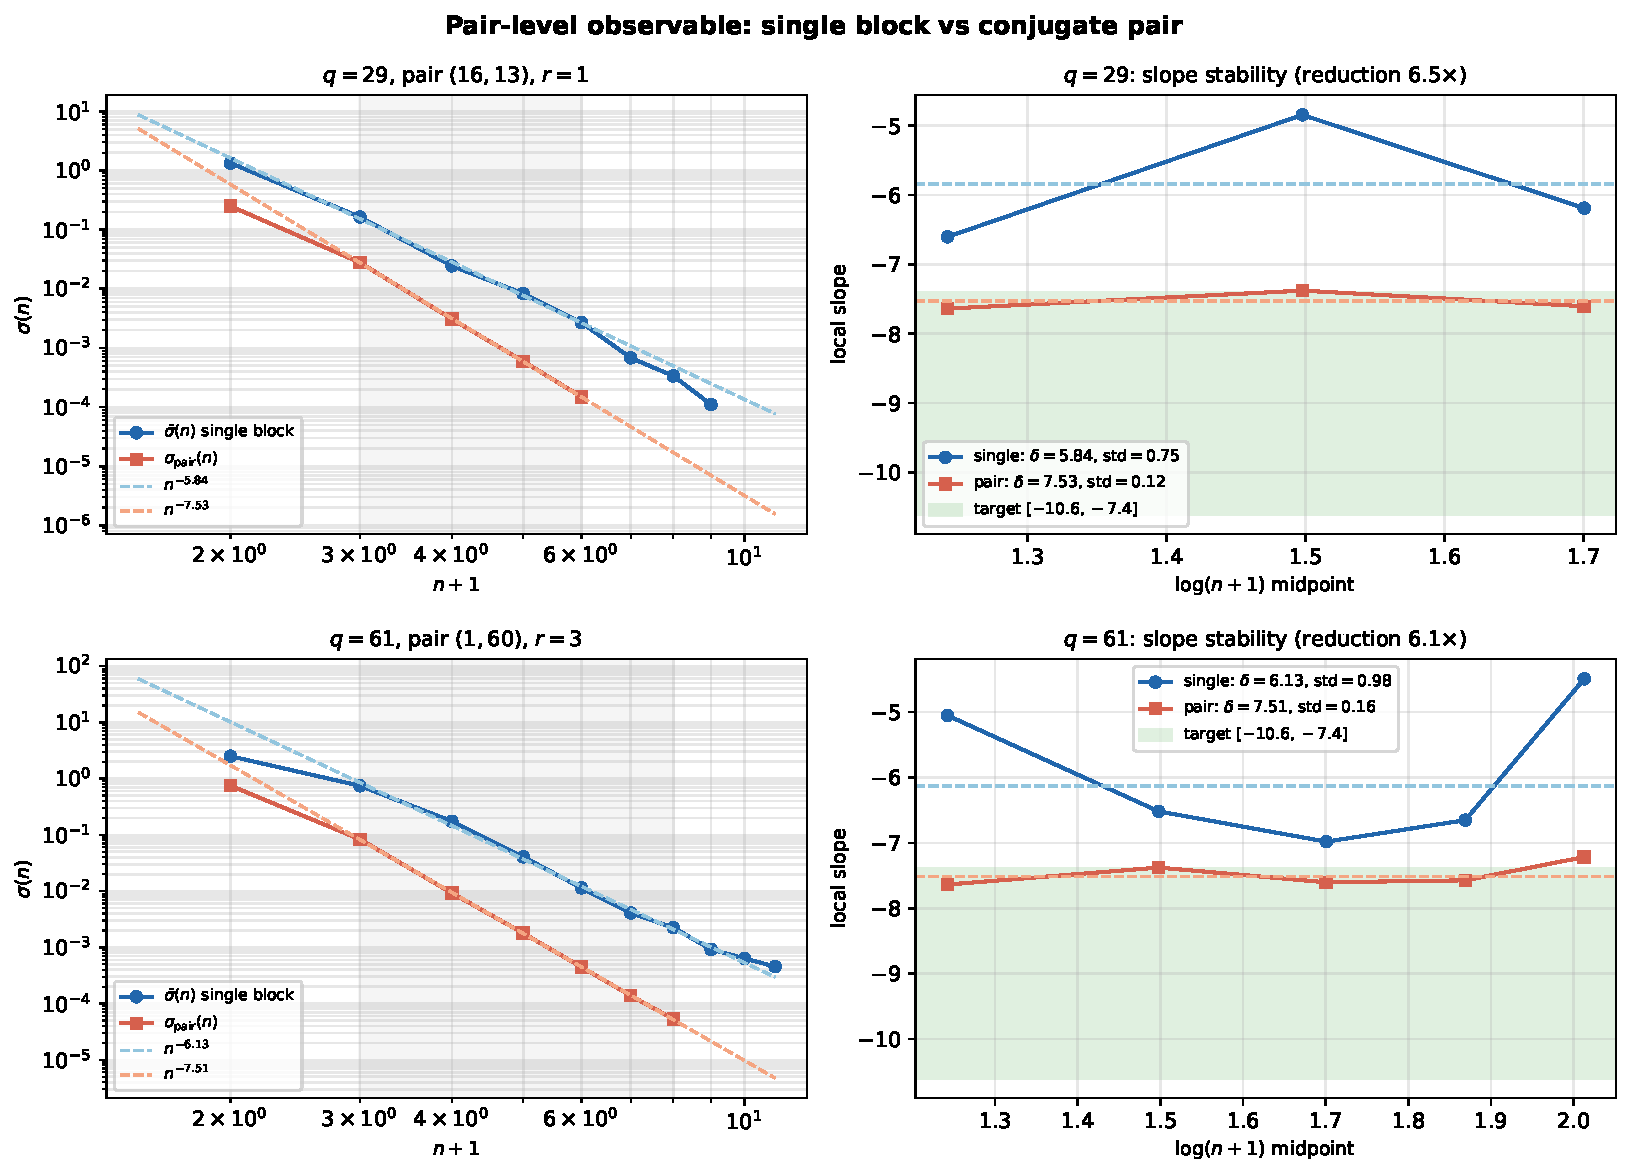
\includegraphics[width=\linewidth]{pair_observable_q29_q61}
\caption{Comparison of single-block and pair-level observables for
$q = 29$ (top row) and $q = 61$ (bottom row).
\emph{Left panels}: log-log profiles of $\bar\sigma(n)$ and
$\sigma_{\mathrm{pair}}(n)$, with power-law fits.
\emph{Right panels}: local log-log slopes in the respective fit
windows $[n_0, n_1]$.
The shaded green band marks the phenomenological target $[-10.6, -7.4]$.
In both cases the pair-level slopes lie entirely within this band,
with variance reduced by a factor~$\sim 6\times$ relative to the
single-block observable.
The power-law scaling becomes well-defined only at the pair level.}
\label{fig:pair_q61}
\end{figure}

\section{Main result and epistemic status}
\label{sec:main}

\begin{proposition}[Fibre admissibility]
\label{prop:main}
Let $\Pi$ carry the parity involution~\eqref{eq:parity}.
In the Weil realisation of $\Heis(\ZqZ)$, the fibres of~$\Pi$
are organised as conjugate pairs $\{c, q-c\}$ under~\eqref{eq:weil_conj}.
The physically relevant observable, defined on complete fibres, is
$\sigma_{\mathrm{pair}}(n) = \sigma_c(n)\,\sigma_{q-c}(n)$,
with asymptotic exponent
$\delta_{\mathrm{pair}} = 2\,\delta_c \approx 7.44$,
consistent with the phenomenological range $[7.4, 10.6]$.
\end{proposition}

\begin{remark}[What is derived vs.\ what is hypothesised]
\label{rem:status}
The following chain is derived: identity~\eqref{eq:weil_conj} is exact
representation theory; Proposition~\ref{prop:sigma_ratio} is a
numerical consequence verified to machine precision;
equation~\eqref{eq:doubling} follows by differentiation.
The identification of conjugate pairs with the fibres of~$\Pi$ is a
structurally motivated hypothesis, consistent with the Born--Infeld
non-injectivity but not yet derived from first principles within
the full Cosmochrony framework.
\end{remark}

\begin{remark}[Absence of model modification]
This result requires no modification of the relaxation dynamics,
the Born--Infeld saturation mechanism, or the Weil-block pipeline.
The underlying model of O12--O15 is unchanged.
The correction is entirely at the level of observable identification:
the correct unit of admissibility is the conjugate pair, not the
individual block.
\end{remark}

\begin{remark}[Amplitude factor $r(c,q)$]
The integer $r(c,q) \in \{1,2,3,4\}$ shifts the amplitude of
$\sigma_{\mathrm{pair}}$ without affecting the
exponent~$\delta_{\mathrm{pair}}$.
It is physically inert for mass-scale extraction.
Its arithmetic origin~---~likely related to quadratic Gauss sums
and character multiplicities of the Weil representation~---~is
an open problem.
\end{remark}

\section{Implications for the O-series programme}
\label{sec:implications}

\paragraph{Corrected pipeline.}
The O12/O13 pipeline should be modified to sample conjugate pairs
$(c, q-c)$ rather than individual blocks.
For each pair, compute $\sigma_c(n) \cdot \sigma_{q-c}(n)$ and
extract~$\delta$ from the resulting profile.
The expected value is $\delta_{\mathrm{pair}} \approx 7.5$,
within the phenomenological target.

\paragraph{Relation to O15 scenarios.}
The C1 scenario of O15 (same functional form, corrected exponent)
is confirmed: $\sigma_{\mathrm{pair}}(n)$ follows the same power-law
form as $\sigma_c(n)$, with exponent doubled by the fibre structure.
The C2 scenario (modified functional form with $q$-dependent correction)
is not required.

\paragraph{Relation to $\bstar$.}
The structural relation $\bstar = 1/(\delta + 1/2)$, used throughout
the O-series, should now be evaluated at
$\delta = \delta_{\mathrm{pair}} \approx 7.44$ rather than at
$\dhat_{\mathrm{exact}} \approx 3.72$.
Since $\bstar$ is defined from the asymptotic scaling of the
physically relevant observable, the substitution
$\delta \to \delta_{\mathrm{pair}}$ is required once admissibility
is defined at the fibre level: the exponent entering the relation
must be that of $R_n^{\mathrm{pair}}$, not of the individual-block
mean~$\bar\sigma(n)$.
This gives
\begin{equation}
\bstar \;\approx\; \frac{1}{7.44 + 0.5} \;\approx\; 0.127,
\end{equation}
compared to the previous estimate $\bstar \approx 0.213$ from
$\delta \approx 3.72$.
The phenomenological implications are deferred to the companion
white paper~\cite{Beau2026a1}.

\paragraph{Open direction.}
A derivation of the parity involution~\eqref{eq:parity} from first
principles within Cosmochrony would close the remaining logical gap
and promote Proposition~\ref{prop:main} from a well-supported
structural result to a theorem.

\section*{Acknowledgements}

The author thanks the extended discussions within the Cosmochrony
programme that led to the identification of the fibre structure
as the relevant unit of admissibility.

\bibliographystyle{plain}
\begin{thebibliography}{99}
% White paper
\bibitem{Cosmochrony}
J.~Beau,
``Cosmochrony: A Pre-Geometric Relational Framework for Emergent Physics,''
white paper, Zenodo (2025).
DOI: \href{https://doi.org/10.5281/zenodo.17957509}{10.5281/zenodo.17957509}.

% Born-Infeld
\bibitem{Beau2026c}
J.~Beau,
``Emergent Spacetime Geometry from Bounded Relational Relaxation,''
companion paper, Zenodo (2026).
DOI: \href{https://doi.org/10.5281/zenodo.18407505}{10.5281/zenodo.18407505}.

% Admissibility
\bibitem{Beau2026a1}
J.~Beau,
``Spectral Admissibility under Bounded Flux: Non-Abelian Mode Selection on Cayley Graphs of SU(2) Subgroups,''
spectral admissibility subprogram paper, Zenodo (2026).
DOI: \href{https://doi.org/10.5281/zenodo.18944985}{10.5281/zenodo.18944985}.

% Capacity
\bibitem{Beau2026a2}
J.~Beau,
``Spectral Capacity Functional and the Binary-Polyhedral Maximality Conjecture,''
spectral admissibility subprogram paper, Zenodo (2026).
DOI: \href{https://doi.org/10.5281/zenodo.18945273}{10.5281/zenodo.18945273}.

% Stratigraphy
\bibitem{Beau2026a4}
J.~Beau,
``Three Particle Generations and Mass Hierarchy from Spectral Stratigraphy,''
spectral admissibility subprogram paper, Zenodo (2026).
DOI: \href{https://doi.org/10.5281/zenodo.19040490}{10.5281/zenodo.19040490}.

% relaxation
\bibitem{Beau2026a5}
J.~Beau,
``Asymptotic Saturation of Projective Resolution: Expander Relaxation Graphs,''
spectral admissibility subprogram paper, Zenodo (2026).
DOI: \href{https://doi.org/10.5281/zenodo.19056975}{10.5281/zenodo.19056975}.

% O1
\bibitem{Beau2026a6}
J.~Beau,
``Projective Resolution Dynamics on Variable-Valence Relaxation Graphs,''
O1 spectral admissibility subprogram paper, Zenodo (2026).
DOI: \href{https://doi.org/10.5281/zenodo.19076319}{10.5281/zenodo.19076319}.

% O3
\bibitem{Beau2026a7}
J.~Beau,
``Projective Dynamics and Mass Hierarchy: Hierarchical Amplification via Growing Relational Valence,''
O3 spectral admissibility subprogram paper, Zenodo (2026).
DOI: \href{https://doi.org/10.5281/zenodo.19076244}{10.5281/zenodo.19076244}.

% O4
\bibitem{Beau2026a8}
J.~Beau,
``Subdiffusive Valence Growth under Bounded Relational Flux: Structural Derivation of the Cascade Exponent $\beta$,''
O4 spectral admissibility subprogram paper, Zenodo (2026).
DOI: \href{https://doi.org/10.5281/zenodo.19101472}{10.5281/zenodo.19101472}.

% O5
\bibitem{Beau2026a9}
J.~Beau,
``Admissible Frontier Saturation and the Cascade Exponent: A Representation-Theoretic Obstruction and its Matrix-Level
Refinement,''
O5 spectral admissibility subprogram paper, Zenodo (2026).
DOI: \href{https://doi.org/10.5281/zenodo.19120328}{0.5281/zenodo.19120328}.

% O6
\bibitem{Beau2026a10}
J.~Beau,
``Matrix-Level Dynamic Redundancy and the Structural Confinement of the Cascade Exponent~$\beta$,''
O6 spectral admissibility subprogram paper, Zenodo (2026).
DOI: \href{https://doi.org/10.5281/zenodo.19140624}{10.5281/zenodo.19140624}.

% O7
\bibitem{Beau2026a11}
J.~Beau,
``Projective Capacity and the Continuum Limit of Admissible Redundancy,''
O7 spectral admissibility subprogram paper, Zenodo (2026).
DOI: \href{https://doi.org/10.5281/zenodo.19149773}{10.5281/zenodo.19149773}.

% O8
\bibitem{Beau2026a12}
J.~Beau,
``Three-Step Path Fingerprints on LPS Graphs and the Capacity Growth Exponent,''
08 spectral admissibility subprogram paper, Zenodo (2025).
DOI: \href{https://doi.org/10.5281/zenodo.19151769}{10.5281/zenodo.19151769}.

% O9
\bibitem{Beau2026a13}
J.~Beau,
``Projective Capacity Beyond Expanders: Polynomial-Growth Relaxation Graphs and the Capacity Exponent,''
09 spectral admissibility subprogram paper, Zenodo (2026).
DOI: \href{https://doi.org/10.5281/zenodo.19154517}{10.5281/zenodo.19154517}

% O10
\bibitem{Beau2026a14}
J.~Beau,
``Polynomial-Growth Capacity Dynamics at Large $q$: Volumetric Growth Confirmation, Capacity Decay, and the Weil
Decomposition Roadmap,''
010 spectral admissibility subprogram paper, Zenodo (2026).
DOI: \href{https://doi.org/10.5281/zenodo.19161074}{10.5281/zenodo.19161074}

% O11
\bibitem{Beau2026a15}
J.~Beau,
``Weil-Block Projective Capacity on Heisenberg Graphs: Resolving the Representation Obstruction and Extracting the
Capacity Exponent,''
011 spectral admissibility subprogram paper, Zenodo (2026).
DOI: \href{https://doi.org/10.5281/zenodo.19169987}{10.5281/zenodo.19169987}

% 012
\bibitem{Beau2026a16}
J.~Beau,
``Exact Weil-Block Projective Capacity on Heisenberg Graphs: Resolving the Final Obstruction to $\delta$ Extraction,''
O12 spectral admissibility subprogram paper, Zenodo (2026).
DOI: \href{https://doi.org/10.5281/zenodo.19194798}{10.5281/zenodo.19194798}.

% 013
\bibitem{Beau2026a17}
J.~Beau,
``Asymptotic Stability of Exact Weil-Block Capacity on Heisenberg Graphs: Extended Prime Range, Variance Reduction,
and Requalification of the \(\delta \to \beta^*\) Tension,''
O13 spectral admissibility subprogram paper, Zenodo (2026).
DOI: \href{https://doi.org/10.5281/zenodo.19210831}{10.5281/zenodo.19210831}.

% O14
\bibitem{Beau2026a18}
J.~Beau,
``Observable-Class Mismatch and the Corrected $\delta \mapsto \bstar$ Relation on Heisenberg Graphs:
Block Normalisation, Central-Phase Contribution,
and Structural Correspondence,''
O14 spectral admissibility subprogram paper, Zenodo (2026).
DOI: \href{https://doi.org/10.5281/zenodo.19226272}{10.5281/zenodo.19226272}.

% Topological invariants
\bibitem{Beau2026k}
J.~Beau,
``Topological Invariants of Admissible Configurations: Charge Quantisation, Absence of Magnetic Monopoles, and Projective Chirality in Cosmochrony,''
compagnon paper, Zenodo (2026).
DOI: \href{https://doi.org/10.5281/zenodo.19282962}{10.5281/zenodo.19282962}.

% O15
\bibitem{Beau2026a19}
J.~Beau,
``Observable-Class Derivation Mismatch and the Exact Growth Equation: From Proxy Capacity to Block-Level Dynamics,''
O15 spectral admissibility subprogram paper, Zenodo (2026).
DOI: \href{https://doi.org/10.5281/zenodo.19281420}{10.5281/zenodo.19281420}.

\end{thebibliography}

\end{document}
